Arduino --- аппаратно-программная платформа <<надстройки>> над микроконтроллерами ATmega, позволяющая быстро и удобно конструировать прототип устройства без необходимости подавать внешнее питание и позволяющая разрабатывать безпаечные макеты.

Arduino представляет собой плату, построенную вокруг ATmega, поддерживающую высокоуровневые инструкции на языке C++, а также предоставляющую удобный интерфейс для программирования через USB-интерфейс. Благодаря большому сообществу и наличию разных библиотек, разработка конечныйх устройств на Arduino представляет собой удобный и быстрый процесс по сравнению с работой непосредственно с микроконтроллером.

Схематика Arduino UNO представлена в приложении A.

Технические характеристики Arduino UNO и Arduino MEGA представлены в таблице~\ref{tab:megatech}~\cite{arduino:mega, arduino:uno}.

\begin{longtable}[c]{|p{2in}|c|c|}
    \caption{Технические характеристики Arduino UNO и Arduino MEGA}
    \label{tab:megatech}\\
    \hline
    \textbf{Параметр} & \textbf{UNO} & \textbf{MEGA}\\
    \hline
    \endfirsthead
    \hline
    \textbf{Параметр} & \textbf{UNO} & \textbf{MEGA}\\
    \hline
    \endhead
        Микроконтроллер & ATmega328 & ATmega2560\\
        \hline
        Оперируемое напряжение & \multicolumn{2}{c|}{5 В}\\
        \hline
        Входное напряжение (реккомендуемое) & \multicolumn{2}{c|}{7 -- 12 В}\\
        \hline
        Входное напряжение (максимальное) & \multicolumn{2}{c|}{6 -- 20 В}\\
        \hline
        Цифровые входы/выходы & 14 (~6) & 54 (~14)\\
        \hline
        Аналоговые входы & 6 & 16\\
        \hline
        Постоянные ток на 1 вход/выход & \multicolumn{2}{c|}{40 мА}\\
        \hline
        Постоянный ток на вход 3.3 В & \multicolumn{2}{c|}{50 мА}\\
        \hline
        Память & 32 Кб & 256 Кб\\
        \hline
        Частота задающего генератора & \multicolumn{2}{c|}{16 МГц}\\
        \hline
\end{longtable}

Условные обозначения элементов на плате Arduino показаны на рисунке~\ref{fig:specuno}.

\begin{figure}[ht]
    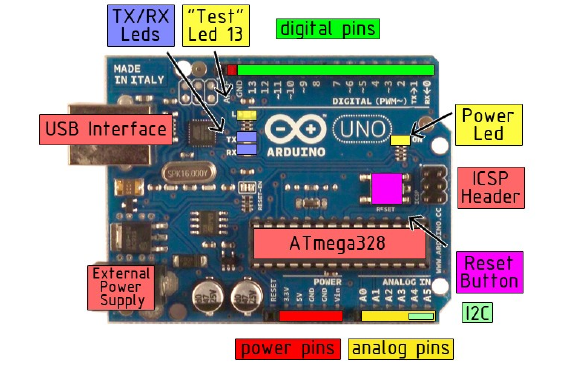
\includegraphics[width=.8\linewidth]{Figures/specuno.png}
    \caption{Спецификация Arduino UNO}
    \label{fig:specuno}
\end{figure}
